A pesquisa adota a Engenharia de Software com desenvolvimento ágil (Scrum) para construção do artefato, organizada em cinco frentes integradas:
(i) modelagem relacional do prontuário;
(ii) \textit{WebApp} de gestão e consulta de pacientes;
(iii) agente escriba do tipo \textit{overhearing}, contemplando transcrição autorizada da consulta em andamento e sugestão de preenchimentos e condutas sem necessidade de interação explícita;
(iv) motor RAG ancorado nas cartilhas do Ministério da Saúde;
e (v) assistente local de consulta contextual, operado via chat, voltado a responder perguntas explícitas com base no contexto do prontuário e documentos recuperados.

A arquitetura reflete o isolamento dos módulos em três subredes \textit{Docker} (\texttt{frontend-nw}, \texttt{backend-nw} e \texttt{data-nw}), conforme a \textit{stack} detalhada na Seção 3 (Materiais). 

A sanitização de PII e a adoção do modo \textit{zero-trust} seguem o módulo de privacidade descrito anteriormente, fundamentando-se nos requisitos de minimização da LGPD apresentados na Seção 2.
Todo o áudio capturado é processado localmente e descartado ao final da interação.

A Figura~\ref{fig:fluxo_consulta} sintetiza o ciclo de vida da transação da consulta médica, estruturado nas seguintes etapas operacionais:

% \begin{figure}[htbp]
%   \centering
%   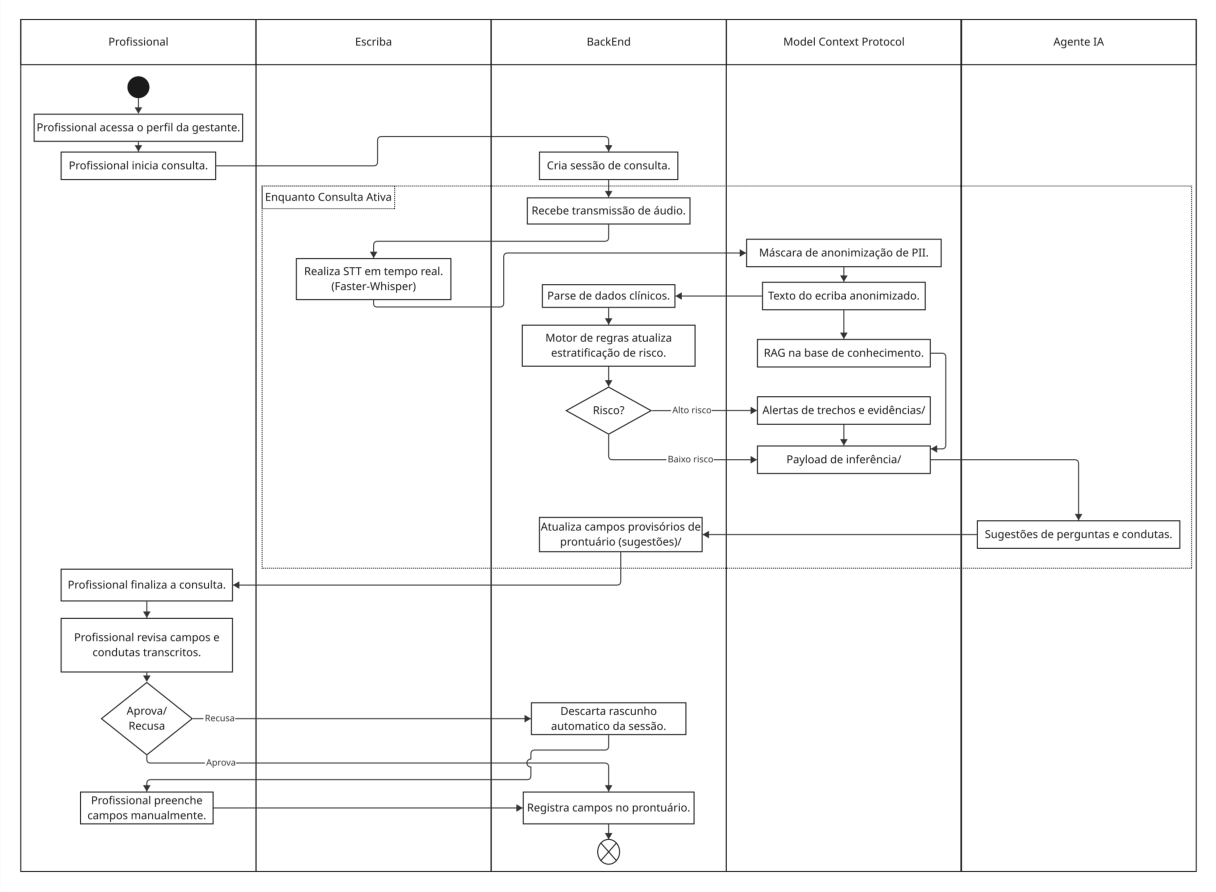
\includegraphics[width=\textwidth, keepaspectratio]{assets/FluxoDeConsulta.pdf}
%   \caption{Pipeline arquitetural e ciclo de vida da transação da consulta médica.}
%   \label{fig:fluxo_consulta}
% \end{figure}

\begin{figure*}[htbp]
  \centering
  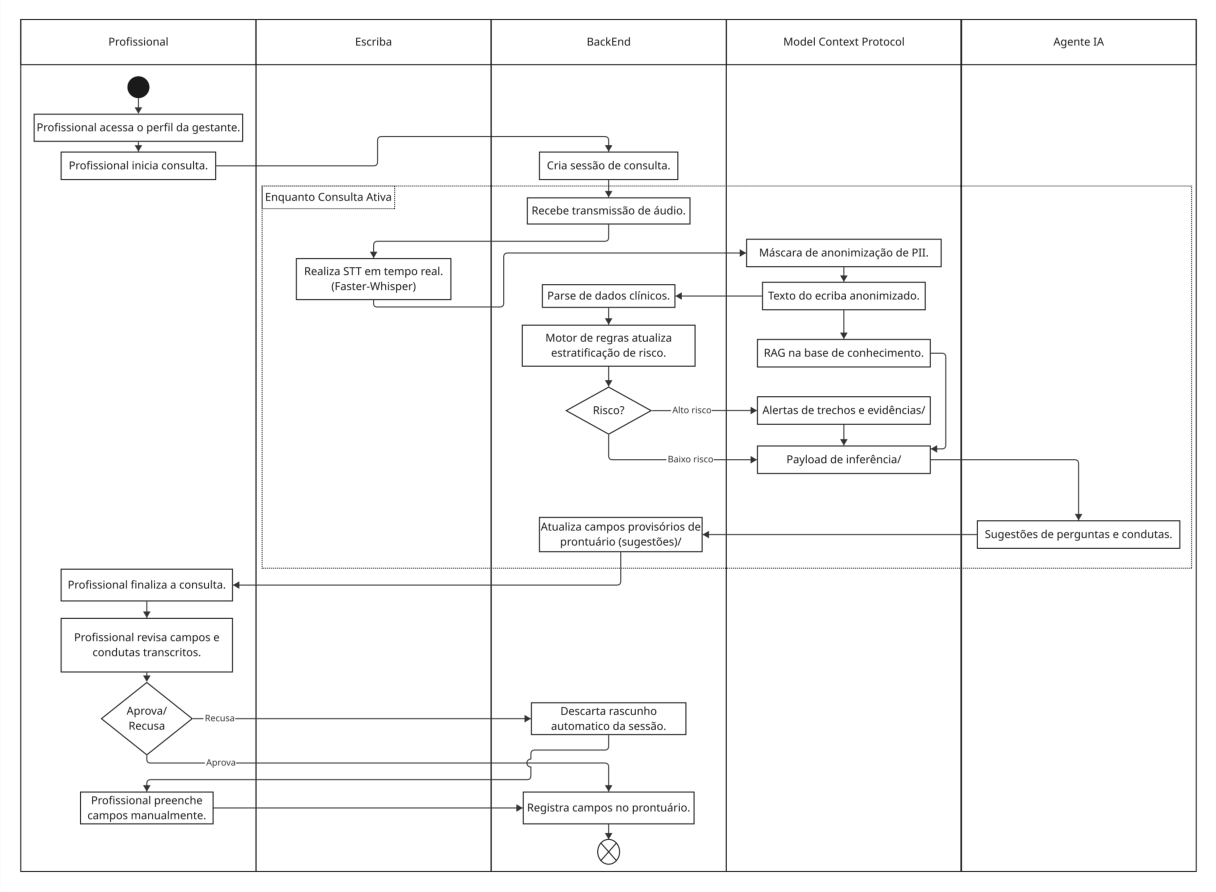
\includegraphics[width=0.8\textwidth]{assets/FluxoDeConsulta.pdf}
  \caption{Pipeline arquitetural e ciclo de vida da transação da consulta médica.}
  \label{fig:fluxo_consulta}
\end{figure*}

\begin{itemize}
  \item \textbf{Captura e transcrição local (STT):} o fluxo de áudio é transcrito em tempo de execução via \textit{Whisper} com diarização.
  \item \textbf{Sanitização de entrada:} o \textit{gateway} remove ou mascara as \textit{PII} na transcrição antes de compor a consulta ao módulo RAG.
  \item \textbf{Recuperação (Retriever):} a busca retorna os trechos relevantes e aplica MMR para diversificar os \textit{chunks} selecionados e reduzir redundâncias no contexto enviado ao modelo.
  \item \textbf{Geração (Generator):} o LLM sintetiza a resposta clínica com hiperparâmetros conservadores, privilegiando a aderência ao contexto recuperado.
  \item \textbf{Apresentação e validação humana:} a interface exibe as sugestões de preenchimento, mantendo a edição manual integralmente disponível.
\end{itemize}

Para cumprir a restrição de segurança clínica, adota-se uma abordagem baseada no conceito de \textit{Human-in-the-Loop}, onde nenhum dado sugerido pela IA é gravado no banco de dados sem a confirmação explícita do profissional (US04), garantindo o controle total sobre o registro.
A principal ameaça à validade interna é a geração de conteúdo não evidenciado nos protocolos da base de conhecimento, sendo esta mitigada por RAG restrito às diretrizes oficiais e \textit{Human-in-the-Loop}.

A ameaça de exposição de \textit{PII} é mitigada por processamento local em um \textit{gateway} de mascaramento aplicado antes da recuperação e inferência.
O anonimizador foi implementado em arquitetura híbrida, combinando regras determinísticas de Expressões Regulares (RegEx) para identificadores brasileiros e um módulo de Reconhecimento de Entidades Nomeadas (NER) especializado em português biomédico.
Como modelo de NER, utilizou-se o\linebreak \texttt{OpenMed-PII-Portuguese-SnowflakeMed-Large-568M-v1}~\cite{openmed-pii-2026}.%, disponibilizado no Hugging Face \cite{openmed-pii-2026}.

A modelagem relacional foi derivada da 8ª edição revisada da Caderneta da Gestante, contemplando entidades para paciente, gestação, consultas, sinais vitais, exames, antecedentes, prontuário e registros de atendimento.
O DER completo foi disponibilizado como material suplementar no repositório do projeto.

O módulo de transcrição baseado em Faster-Whisper foi integrado ao protótipo para validar a viabilidade técnica do fluxo de captura local de áudio. Contudo, sua avaliação sistemática não compõe o escopo experimental deste trabalho, permanecendo como etapa futura.